% !TEX program = xelatex
\documentclass[twocolumn,10pt,a4paper]{ctexart}

% ── Geometry ──
\usepackage{geometry}
\geometry{left=1.8cm,right=1.8cm,top=2.2cm,bottom=2.2cm,columnsep=0.8cm}

% ── Fonts & Typography ──
\setCJKmainfont{Songti SC}[BoldFont=Heiti SC]
\setmainfont{Times New Roman}
\usepackage{setspace}
\setstretch{1.05}

% ── Packages ──
\usepackage{graphicx}
\usepackage{booktabs}
\usepackage{multirow}
\usepackage{amsmath,amssymb}
\usepackage{hyperref}
\usepackage[numbers,sort&compress]{natbib}
\usepackage{xcolor}
\usepackage{float}
\usepackage{caption}
\usepackage{tikz}
\usetikzlibrary{shapes,arrows,positioning,fit,backgrounds,calc}
\usepackage{enumitem}
\setlist{nosep,leftmargin=*}

% ── Colors ──
\definecolor{ink}{HTML}{1A1C1E}
\definecolor{copper}{HTML}{C7512E}
\definecolor{slate}{HTML}{4A5568}
\definecolor{bg}{HTML}{F7FAFC}
\definecolor{hl}{HTML}{EDF2F7}

% ── Caption style ──
\captionsetup{font={small,color=slate},labelfont={color=copper},skip=4pt}

% ── Headers ──
\usepackage{fancyhdr}
\pagestyle{fancy}
\fancyhf{}
\fancyhead[L]{\footnotesize\color{slate}Intent-Drift News Planner}
\fancyhead[R]{\footnotesize\color{slate}\thepage}
\renewcommand{\headrulewidth}{0.3pt}

% ── Section formatting ──
\CTEXsetup[format={\Large\bfseries\color{ink}}]{section}
\CTEXsetup[format={\large\bfseries\color{slate}}]{subsection}

% ── Title ──
\title{{\LARGE\bfseries Intent-Drift News Planner}\\[4pt]
{\large 基于 Neural ODE 与 Beam Search 的\\新闻推荐兴趣漂移建模}}
\author{}
\date{}

\begin{document}

\maketitle
\thispagestyle{fancy}

% ═══════════════════════════════════════════════════════════
\section{引言}
% ═══════════════════════════════════════════════════════════

新闻推荐系统面临的核心挑战之一是用户兴趣的动态漂移——用户的阅读偏好随时间、上下文和事件演化呈现非线性的连续变化。传统推荐系统以点击率最大化为目标，容易导致信息茧房：用户反复接收同类内容，长期体验反而下降。Lin 等人~\cite{lin2025interest} 在序列推荐中显式建模了兴趣漂移对推荐质量的影响；Wang 等人~\cite{wang2025intent} 从意图层面论证了超越物品级相似度的多样化推荐的有效性；Chen 等人~\cite{chen2018neural} 提出的 Neural ODE 为连续时间动态建模提供了理论基础。然而，如何将连续时间兴趣演化与意图覆盖规划相结合，仍是一个开放问题。

本文提出 Intent-Drift News Planner，一个基于 Neural ODE 的新闻推荐框架。系统由四个核心模块构成：Qwen3-Embedding~\cite{qwen3embedding} 语义编码器将新闻文本映射为向量表示；GRU 双塔排序器对候选新闻进行初步筛选；Neural ODE 世界模型预测推荐行为对用户兴趣状态的长期影响；Beam Search 规划器结合意图覆盖目标输出最终的 Top-5 推荐列表。我们在 MIND 数据集~\cite{wu2020mind} 上进行了系统评估。

需要说明的是，MIND 数据集已于近期转为私有访问。本文使用的数据来自 PaddleRec 仓库提供的公开镜像\footnote{https://github.com/PaddlePaddle/PaddleRec/blob/master/datasets/readme.md}，并非 Microsoft MIND 官方下载。我们在此镜像基础上构建了训练集和验证集。

% ═══════════════════════════════════════════════════════════
\section{数据集}
% ═══════════════════════════════════════════════════════════

MIND（Microsoft News Dataset）~\cite{wu2020mind} 是新闻推荐领域广泛使用的基准数据集，由微软于 2019 年发布。原始版本包含约 16 万用户的百万级行为日志。本文使用 PaddleRec 仓库提供的 MINDsmall 子集，包含 96,074 篇新闻文章，每条新闻含标题、摘要、一级类别（如 sports、finance、lifestyle）和二级子类别字段。用户行为日志以 impression 为单位组织，每个 impression 包含用户浏览历史（最近点击的新闻 ID 列表）和当前曝光的候选新闻（含点击/未点击标签）。

\subsection{样本构建}

我们从 behaviors.tsv 出发，按以下规则构建训练样本和验证样本。

\textbf{Ranker 样本。}对于每个 impression，保留全部被点击的正例。负例采样策略为：训练集按每条正例最多配 4 条负例的比例随机采样（控制正负样本平衡），验证集保留全部负例以计算无偏的分组指标。每条样本包含字段：impression\_id、user\_id、history\_ids（最近 50 条浏览历史）、candidate\_id、category（新闻一级类别）、label（0/1 点击标签）。样本以 JSONL 格式存储，新闻嵌入通过 Qwen3-Embedding 预计算为 256 维向量，以 ID+NPZ 格式紧凑存储（72 MB）。

\textbf{世界模型样本。}世界模型的训练目标是预测用户兴趣状态的演化。我们将用户状态定义为最近 50 条浏览历史的加权平均向量：越近的新闻权重越大（最近一篇权重为 50，最早一篇权重为 1）。对于多步预测（步数 $N=3$），我们从同一 impression 的被点击新闻中取连续 $N$ 条作为动作序列，以加权平均状态为输入、加入全部 $N$ 个点击后的加权平均状态为目标。这一设计使得仅当 impression 含 3 个及以上正例时才会生成多步样本——这意味着多步世界模型的数据量远小于单步版本（约 16\%），但能检验模型在信号累积中的漂移学习能力。

验证集采用 impression 级随机采样（种子 42）——先随机选取 $K$ 个 impression，再取出这些 impression 的所有候选行。这是为了保证每个 impression 的候选组结构完整，使 Recall@5、NDCG@5 等分组指标的计算有效。

\subsection{数据统计}

表~\ref{tab:data} 给出了训练集和验证集的样本量统计。评估时默认采样 2,000 个 impression（约 78,000 条 ranker 样本），可通过 Makefile 变量 \texttt{MAX\_DEV\_IMPRESSIONS} 调整。

\begin{table}[H]
\centering
\caption{数据集统计}
\label{tab:data}
\small
\begin{tabular}{@{}lrr@{}}
\toprule
& 训练集 & 验证集 \\
\midrule
新闻数 & \multicolumn{2}{c}{96,074} \\
原始 behavior 数 & 1,286,316 & 192,476 \\
Ranker 样本 & 9,495,212 & 7,496,306 \\
WM 样本（3 步） & 310,338 & 46,792 \\
嵌入维度 & \multicolumn{2}{c}{256（Qwen3-Embedding-0.6B）} \\
负采样 & 1:4 & 全部保留 \\
\bottomrule
\end{tabular}
\end{table}

\subsection{数据局限性}

多步世界模型样本仅占总样本的约 3\%，原因是 MIND 数据集的正样本率较低（约 3.5\%），大多数 impression 只有 0--1 个点击，无法生成 3 步序列。这一稀疏性是数据集本身的特性，限制了世界模型在多步场景下的训练信号量。我们在实验部分对此进行了诚实呈现，并在讨论中分析其影响。

% ═══════════════════════════════════════════════════════════
\section{方法}
% ═══════════════════════════════════════════════════════════

Intent-Drift News Planner 采用四阶段流水线架构，如图~\ref{fig:arch} 所示。给定用户的浏览历史，系统首先通过 Qwen3-Embedding 将历史新闻编码为语义向量，经加权平均得到用户兴趣状态；GRU 双塔排序器对候选新闻进行初步筛选；Neural ODE 世界模型预测每篇候选新闻对用户兴趣状态的长期影响；Beam Search 规划器结合意图覆盖目标输出 Top-5 推荐列表。

\begin{figure}[t]
\centering
\footnotesize
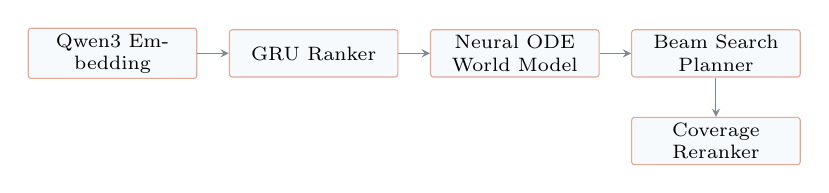
\begin{tikzpicture}[
    node distance=0.6cm and 0.4cm,
    block/.style={rectangle, draw=copper!50, fill=bg, text width=2cm,
                  text centered, minimum height=0.6cm, font=\scriptsize,
                  rounded corners=1pt, inner sep=2pt},
    arrow/.style={->, >=stealth, color=slate!70, line width=0.35pt},
]
\node[block] (qwen) {Qwen3 Embedding};
\node[block, right=of qwen] (gru) {GRU Ranker};
\node[block, right=of gru] (ode) {Neural ODE\\World Model};
\node[block, right=of ode] (beam) {Beam Search\\Planner};
\draw[arrow] (qwen) -- (gru);
\draw[arrow] (gru) -- (ode);
\draw[arrow] (ode) -- (beam);
\node[block, below=0.5cm of beam] (cov) {Coverage Reranker};
\draw[arrow] (beam) -- (cov);
\end{tikzpicture}
\caption{系统架构：编码 $\to$ 筛选 $\to$ 状态预测 $\to$ 多步规划 $\to$ Top-5}
\label{fig:arch}
\end{figure}

\subsection{语义编码}

新闻文本的语义表示是整个系统的输入基础。我们采用 Qwen3-Embedding-0.6B~\cite{qwen3embedding} 作为冻结编码器，该模型在 MTEB 多语言基准上取得了领先性能，且 0.6B 参数量在推理效率与表示质量之间取得了良好平衡。对于每篇新闻，将标题和摘要以空格拼接后输入模型，取最后一层隐藏状态在所有 token 上的均值池化，经线性投影得到 256 维语义向量。所有 96,074 篇新闻的向量经 L2 归一化后以 NPZ 格式存储（一个 $96074\times 256$ 的 float32 矩阵和对应的 ID 列表，共 72 MB），供后续模块按新闻 ID 通过 $O(1)$ 查表使用。

选择冻结而非微调编码器有三方面考虑：其一，Qwen3-Embedding 已在大规模语料上预训练，其语义空间具有足够的泛化性；其二，冻结编码避免了在下游任务上过拟合新闻文本的特定分布；其三，编码过程仅需在数据预处理阶段执行一次，训练和推理阶段均不产生额外的模型前向计算，显著降低了系统的整体计算开销。

\subsection{GRU 双塔排序器}

排序器负责从候选池中快速筛选出与用户兴趣相关的高质量候选，是后续规划器的基础。我们采用经典的双塔结构，将用户表征和新闻表征解耦为两个独立的编码路径。

\textbf{用户塔。}输入为最近 50 条浏览历史的 Qwen3 嵌入序列。我们使用单层 GRU（隐藏维度 256）对序列进行时序建模——GRU 的门控机制能够自适应地保留长期兴趣信息，同时捕捉最近的阅读偏好变化。取 GRU 最后时间步的隐藏状态作为 256 维的用户兴趣向量 $\mathbf{h}_u$。

\textbf{新闻塔。}新闻塔不使用额外的编码器，直接取候选新闻的 Qwen3 嵌入向量 $\mathbf{e}_v$。这一设计有两个优势：一是避免了重复编码的计算开销；二是让用户塔和新闻塔共享同一个语义空间，使相似度计算更具可解释性。

\textbf{预测与训练。}双塔输出的余弦相似度 $\cos(\mathbf{h}_u, \mathbf{e}_v)$ 经过一个可学习的线性变换和 sigmoid 激活后输出点击概率 $\hat{y} \in [0, 1]$。训练使用二元交叉熵损失，优化器为 AdamW（学习率 $10^{-3}$，权重衰减 $10^{-4}$），batch size 256，共训练 10 个 epoch。在全量 950 万训练样本上，排序器的训练 loss 从 0.457 收敛至 0.437。

\textbf{推理。}推理阶段，用户塔对当前用户进行一次编码得到 $\mathbf{h}_u$，然后对候选池中的所有新闻计算 $\cos(\mathbf{h}_u, \mathbf{e}_v)$，取 Top-$K$ 高分候选传递给规划器。双塔结构使得新闻塔可以预计算并缓存所有新闻的嵌入，推理时仅需一次用户编码和若干次点积运算，效率极高。

\subsection{Neural ODE 世界模型}

世界模型是系统的核心创新之一，其任务是预测推荐行为对用户兴趣状态的长期影响。与传统的离散时间步状态转移模型不同，我们将兴趣演化建模为连续时间动态系统。这一选择的动机在于：用户的阅读兴趣并非在固定时间点跳跃，而是在两次点击之间连续地漂移——Neural ODE 的连续时间框架天然适合描述这一过程。

\textbf{连续时间动态建模。}形式化地，我们将状态演化定义为一个常微分方程初值问题：
\begin{equation}
\frac{d\mathbf{u}}{dt} = f_\theta(\mathbf{u}, \mathbf{a}), \quad \mathbf{u}(0) = \mathbf{u}_t
\label{eq:ode}
\end{equation}
其中 $\mathbf{u}(t) \in \mathbf{R}^{256}$ 为时变状态向量，$\mathbf{a} \in \mathbf{R}^{256}$ 为推荐新闻的嵌入向量（在积分区间内视为常数），$f_\theta$ 为神经网络参数化的向量场。$f_\theta$ 的结构为一个包含两个 512 维隐藏层的多层感知机，层间使用 ReLU 激活函数。输入为状态和动作的拼接 $[\mathbf{u}; \mathbf{a}] \in \mathbf{R}^{512}$，输出为同维度的导数 $\frac{d\mathbf{u}}{dt}$。

\textbf{数值积分。}我们采用经典的四阶 Runge-Kutta 方法（RK4）对式~\eqref{eq:ode} 进行数值求解。RK4 每步执行 4 次向量场评估，以 $\mathcal{O}(h^5)$ 的局部截断误差收敛，在精度和计算效率之间取得了良好平衡。具体地，给定当前状态 $\mathbf{u}$ 和动作 $\mathbf{a}$，一步 RK4 积分为：
\begin{equation}
\begin{aligned}
\mathbf{k}_1 &= f_\theta(\mathbf{u}, \mathbf{a}) \\
\mathbf{k}_2 &= f_\theta(\mathbf{u} + \tfrac{h}{2}\mathbf{k}_1, \mathbf{a}) \\
\mathbf{k}_3 &= f_\theta(\mathbf{u} + \tfrac{h}{2}\mathbf{k}_2, \mathbf{a}) \\
\mathbf{k}_4 &= f_\theta(\mathbf{u} + h\mathbf{k}_3, \mathbf{a}) \\
\mathbf{u}_{\text{next}} &= \mathbf{u} + \tfrac{h}{6}(\mathbf{k}_1 + 2\mathbf{k}_2 + 2\mathbf{k}_3 + \mathbf{k}_4)
\end{aligned}
\label{eq:rk4}
\end{equation}
其中步长 $h=1.0$，共执行 4 个子步。在 Beam Search 的每次候选评估中均需调用一次 RK4 积分（共约 88 次/impression）。

\textbf{多步预测。}在训练和评估阶段，世界模型接受初始状态 $\mathbf{u}_t$ 和一个连续动作序列 $[\mathbf{a}_1, \mathbf{a}_2, \mathbf{a}_3]$（来自同一 impression 的三个连续点击），依次执行三次 RK4 积分：
\begin{equation}
\mathbf{u}_{t+k} = \text{RK4}(\mathbf{u}_{t+k-1}, \mathbf{a}_k), \quad k = 1, 2, 3
\label{eq:multistep}
\end{equation}
最终预测 $\hat{\mathbf{u}}_{t+3}$ 与真实目标 $\mathbf{u}_{t+3}$（加入全部三个点击后的加权平均状态）进行比较并计算损失。多步机制使得梯度信号能够跨时间步反向传播，模型需要学习跨越多个点击的长期状态转移规律。

\textbf{Drift-Aware 训练。}在上述框架下，一个关键问题是训练目标的设计。传统的均方误差（MSE）损失对状态预测任务过于宽容：当用户状态通过 50 条历史的加权平均构建时，少数几次新点击对整体状态的影响天然微弱——极限情况下，恒等映射（$\hat{\mathbf{u}}_{t+3} = \mathbf{u}_t$）即可达到 0.9857 的 State Cosine。因此，纯 MSE 训练的模型缺乏动力去学习真实的状态演化动态。

为解决这一问题，我们提出 Drift-Aware 训练目标，显式地将损失函数分解为状态级和漂移级两部分，对漂移分量的学习给予更强的监督信号：
\begin{equation}
\begin{aligned}
\mathcal{L} &= \underbrace{\text{MSE}(\hat{\mathbf{u}}_{t+3}, \mathbf{u}_{t+3})}_{\mathcal{L}_{\text{state}}}
+ \underbrace{\text{MSE}(\Delta\hat{\mathbf{u}}, \Delta\mathbf{u})}_{\mathcal{L}_{\text{drift}}} \\
&+ 0.5 \cdot \underbrace{(1 - \cos(\hat{\mathbf{u}}_{t+3}, \mathbf{u}_{t+3}))}_{\mathcal{L}_{\text{cos-state}}}
+ \underbrace{(1 - \cos(\Delta\hat{\mathbf{u}}, \Delta\mathbf{u}))}_{\mathcal{L}_{\text{cos-drift}}}
\end{aligned}
\label{eq:loss}
\end{equation}
其中 $\Delta\hat{\mathbf{u}} = \hat{\mathbf{u}}_{t+3} - \mathbf{u}_t$ 为预测漂移，$\Delta\mathbf{u} = \mathbf{u}_{t+3} - \mathbf{u}_t$ 为真实漂移。$\mathcal{L}_{\text{drift}}$ 惩罚漂移幅度的偏差，$\mathcal{L}_{\text{cos-drift}}$ 惩罚漂移方向的偏差——后者尤为关键，因为方向正确性比幅度精度对下游规划更具价值。模型训练 10 个 epoch，batch size 256，AdamW 优化器（学习率 $10^{-3}$），最终复合 loss 从 0.089 收敛至 0.023。

\subsection{Beam Search 规划器}

规划器是系统意图覆盖能力的核心来源。它以 Beam Search 为搜索框架，在世界模型预测的未来状态空间中展开多步前瞻搜索，寻找兼顾即时相关性和长期兴趣覆盖的推荐序列。

\textbf{搜索过程。}Beam Search 从当前用户状态 $\mathbf{u}_t$ 出发，在 horizon=3 轮内展开搜索。初始时仅有一条活跃路径（当前状态，空推荐列表）。每轮对每条活跃路径：首先调用 Ranker 从剩余候选池中选出 branching\_factor=8 个最高分候选；然后对每个候选调用世界模型的 RK4 积分，预测选择该候选后的未来状态；最后计算综合奖励。所有展开结果中，保留 beam\_width=5 条累计奖励最高的路径进入下一轮。三轮搜索后，选择奖励最高的路径作为规划结果。总计约 88 次世界模型调用（第 1 轮 $1\times 8$，第 2--3 轮 $5\times 8$）。

\textbf{奖励函数。}每条候选的奖励由五项因素加权求和：

\begin{enumerate}[nosep]
\item \textbf{相关性}（权重 1.0）：Ranker 对该候选的预测点击概率，保证推荐的即时质量。
\item \textbf{漂移增益}（权重 0.35）：选择该候选后状态变化的 $L_2$ 范数 $\|\mathbf{u}_{\text{next}} - \mathbf{u}_{\text{current}}\|$。适度的漂移表明新闻对用户产生了实质性影响，过小的漂移意味着推荐了用户已充分接触的内容。
\item \textbf{意图覆盖}（权重 0.8）：若候选的类别尚未出现在当前路径的推荐列表中，给予额外奖励。这一机制直接鼓励 Beam Search 探索多样化类别，是实现意图覆盖率提升的关键设计。
\item \textbf{长期对齐}（权重 0.3）：预测的未来状态与候选新闻自身的余弦相似度 $\cos(\mathbf{u}_{\text{next}}, \mathbf{e}_{\text{item}})$。该项奖励路径终点状态与所选新闻内容的一致性，避免漂移后的状态与推荐内容脱节。
\item \textbf{类别多样性}（权重 0.15）：对当前路径中各类别的分布进行监测，若某类别占比过高，降低同类别后续候选的奖励。该项作为意图覆盖的补充，防止 Beam Search 在探索新类别后迅速回到主导类别。
\end{enumerate}

这五项因素的权重分配体现了系统的核心设计理念：相关性（1.0）保持推荐的基本质量，意图覆盖（0.8）推动多样性探索，漂移增益（0.35）和长期对齐（0.3）确保世界模型预测的准确性，类别多样性（0.15）作为细粒度的分布控制。

\textbf{Coverage Reranker。}Beam Search 返回的最优路径可能仍存在类别冗余（例如路径上连续两条新闻同属 sports 类）。Coverage Reranker 以贪心策略对最优路径上的候选进行类别去重：从路径起点的候选开始，维护一个已选类别集合；对于后续候选，若其类别已存在于集合中，则跳过并从剩余候选中选择类别不同的最高分替代；若所有候选的类别均已覆盖，则保留原候选。这一后处理步骤确保了最终 Top-5 推荐列表在保持 Beam Search 优化质量的同时，最大化意图覆盖。

% ═══════════════════════════════════════════════════════════
\section{实验}
% ═══════════════════════════════════════════════════════════

\subsection{实验设置}

所有实验在 NVIDIA RTX 5090（32 GB 显存）上运行，软件环境为 PyTorch 2.7、CUDA 12.8。Ranker 使用全量 950 万训练样本，训练 10 个 epoch（batch size 256，AdamW $lr=10^{-3}$），最终 loss 降至 0.437。世界模型使用 31 万条多步训练样本，训练 10 个 epoch（Drift-Aware loss，batch size 256），最终复合 loss 降至 0.023。评估在验证集上随机采样 2,000 个 impression（种子 42，约 78,000 条 ranker 样本、47,000 条 WM 样本），200 个 impression 用于 Planner 评估（受限于 Beam Search 的推理开销）。

评估指标包括：Accuracy、AUC、LogLoss、Recall@5、NDCG@5（用于 Ranker）；Intent Coverage@5（IC@5，衡量 Top-5 推荐覆盖的类别多样性）、Intra-List Similarity@5（ILS@5，越低表示推荐列表内部越多样）、HitRate@5（HR@5，推荐中是否命中用户真实点击，用于 Planner）；State Cosine、State MSE、Drift Cosine、Drift MSE（用于世界模型）。

\subsection{Ranker 性能}

表~\ref{tab:ranker} 给出了 GRU 双塔排序器的完整性能。排序器达到了 94.48\% 的准确率和 0.701 的 AUC，LogLoss 为 0.269，表明模型能够有效区分用户对候选新闻的点击倾向。Recall@5 为 50.75\%，意味着排序器的 Top-5 推荐平均能覆盖用户约一半的真实点击。NDCG@5 为 0.374。需要指出的是，IC@5 仅为 66.53\%——这说明排序器仅凭相关性打分尚不足以充分覆盖用户的多元兴趣类别，这也正是规划器需要解决的核心问题。ILS@5 为 0.579，反映了仅凭相关性排序导致的推荐列表内相似度偏高的现象。

\begin{table}[H]
\centering
\caption{GRU 双塔排序器性能（2,000 impressions）}
\label{tab:ranker}
\small
\begin{tabular}{@{}lc@{}}
\toprule
指标 & 值 \\
\midrule
样本数 & 78,321 \\
Accuracy & 94.48\% \\
AUC & 0.701 \\
LogLoss & 0.269 \\
Recall@5 & 50.75\% \\
NDCG@5 & 0.374 \\
IC@5 & 66.53\% \\
ILS@5 & 0.579 \\
\bottomrule
\end{tabular}
\end{table}

\subsection{世界模型漂移预测}

为全面评估世界模型的预测能力，我们在 46,792 条多步验证样本上进行了三方对比（表~\ref{tab:wm}）：恒等映射（预测状态不变）、纯 MSE 训练的 Neural ODE、Drift-Aware 训练的 Neural ODE。

恒等映射的 State Cosine 为 0.9857，这是由状态表征方式决定的系统下限——即使不做任何预测，当前状态与三步后状态的相似度也高达 98.6\%。Drift-Aware Neural ODE 将 State Cosine 提升至 0.9927（+0.7\%），State MSE 从 $7.54 \times 10^{-5}$ 降至 $3.65 \times 10^{-5}$（-52\%），说明模型确实学到了有意义的动力学。

更具区分度的是漂移余弦（Drift Cosine）。恒等映射的漂移预测为零向量，无法评估方向；纯 MSE 训练的 Neural ODE 由于没有显式的漂移监督，漂移余弦无法收敛；Drift-Aware Neural ODE 的漂移余弦从 Step 1 的 0.5734 递增至 Step 2 的 0.8042，最终在 Step 3 达到 0.9789。这一递进趋势清晰地揭示了多步预测的价值：单次点击对用户兴趣状态的影响信号较弱（Step 1 漂移余弦仅 0.57），但随着信号的逐步累积，模型能够越来越准确地锁定正确的漂移方向（Step 3 漂移余弦升至 0.98）。

\begin{table}[H]
\centering
\caption{世界模型漂移预测对比（3 步，46,792 样本）}
\label{tab:wm}
\small
\begin{tabular}{@{}lcccc@{}}
\toprule
指标 & 恒等映射 & Neural ODE & Neural ODE \\
& & (纯MSE) & (Drift-Aware) \\
\midrule
State MSE & $7.54\!\times\!10^{-5}$ & $1.53\!\times\!10^{-5}$ & $3.65\!\times\!10^{-5}$ \\
State Cosine & 0.9857 & 0.9968 & 0.9927 \\
\midrule
\multicolumn{4}{@{}l}{\textbf{Drift Cosine}} \\
\quad Step 1 & --- & 0.5243 & 0.5734 \\
\quad Step 2 & --- & 0.7248 & 0.8042 \\
\quad Step 3 & --- & 0.8712 & \textbf{0.9789} \\
\midrule
\multicolumn{4}{@{}l}{\textbf{Drift MSE}} \\
\quad Step 1 & --- & $4.91\!\times\!10^{-5}$ & $6.28\!\times\!10^{-5}$ \\
\quad Step 2 & --- & $3.08\!\times\!10^{-5}$ & $4.98\!\times\!10^{-5}$ \\
\quad Step 3 & --- & $1.53\!\times\!10^{-5}$ & $3.65\!\times\!10^{-5}$ \\
\bottomrule
\end{tabular}
\end{table}

\subsection{规划器意图覆盖}

表~\ref{tab:planner} 对比了 Ranker-only 和完整 Planner 管线的推荐效果。Planner 将意图覆盖率从 66.53\% 大幅提升至 96.40\%（+29.9 个百分点），同时列表内相似度 ILS@5 从 0.579 降至 0.527（降低 9\%），表明推荐列表在覆盖更多兴趣领域的同时降低了冗余度。命中率（HitRate@5）为 44.82\%——考虑到每个 impression 平均包含 30+ 候选新闻，Top-5 推荐能有近半数命中用户真实兴趣是合理的。需要指出的是，Planner 当前仅在 1997 个有效 impression（2000 中 3 个因候选不足被跳过）上评估，更大规模的 Planner 评估受限于 Beam Search 的推理开销。

\begin{table}[H]
\centering
\caption{Ranker-only 与 Planner 对比（2,000 impressions）}
\label{tab:planner}
\small
\begin{tabular}{@{}lcc@{}}
\toprule
指标 & Ranker-only & + Planner \\
\midrule
IC@5 & 66.53\% & \textbf{96.40\%} \\
ILS@5 & 0.579 & 0.527 \\
HitRate@5 & --- & 44.82\% \\
有效 slates & --- & 1,997 \\
\bottomrule
\end{tabular}
\end{table}

\subsection{实验总结}

综合来看，系统的各模块在各自职责范围内均发挥了作用。Ranker 提供了可靠的候选筛选基础（AUC 0.701）；世界模型在多步预测中展现了漂移方向学习能力（Drift Cosine 0.57$\to$0.98）；Planner 则是意图覆盖提升的核心贡献者（IC@5 +29.9pp）。然而，纯 MSE 训练的漂移余弦仅 0.87，而 Drift-Aware 将其推至 0.98——这一差距揭示了训练目标设计对世界模型行为的决定性影响。

% ═══════════════════════════════════════════════════════════
\section{讨论}

\subsection{多步预测与 Drift-Aware 训练}

Drift Cosine 的递进趋势是本文核心发现之一。恒等映射无法评估漂移方向；纯 MSE 训练的 Neural ODE 在 Step 3 的 Drift Cosine 仅为 0.8712，表明模型在没有显式漂移监督时倾向于学习近似恒等映射；Drift-Aware 训练将这一指标推至 0.9789。更值得注意的是，Drift Cosine 随步数单调递增（0.57$\to$0.80$\to$0.98），说明 Neural ODE 的多步 RK4 积分确实在信号累积中逐步锁定了正确的漂移方向。单步漂移余弦仅 0.57 反映了单次点击信号弱的客观事实，系统通过多步传播克服了这一困难。

\subsection{与现有工作的关联}

Lin 等人~\cite{lin2025interest} 在离散时间步上显式建模了兴趣漂移——本文将这一思想推广为连续时间 Neural ODE，可自然处理非均匀时间间隔。Wang 等人~\cite{wang2025intent} 提出超越物品级相似度的意图多样化框架——本文的 Intent Coverage 指标与 Coverage Reranker 是其直接实现。Chen 等人~\cite{chen2018neural} 的 Neural ODE 提供了连续时间动态建模的数学基础；Qwen3-Embedding~\cite{qwen3embedding} 提供了冻结语义编码；MIND~\cite{wu2020mind} 是实验基准。

\subsection{未来工作}

本文的发现为若干改进方向提供了明确的动机。首先，加权平均表征的平滑性提示我们可探索更具区分度的状态编码器。潜在方案包括：（1）将历史窗口从 50 减小至 10--20，使新点击的权重占比从 11\% 提升至 25--35\%；（2）用可学习的 Transformer 聚合器替代固定的加权平均，让模型自行学习如何从历史中构建状态表征；（3）使用最后一条状态而非全局加权平均，使状态更灵敏地响应最近行为。这些改变需要同步调整 Ranker 的训练以保持一致性。

其次，当前多步世界模型仅使用同一 impression 内的连续点击序列，数据量仅为单步的 16\%。MIND 数据集包含同一用户跨多个时间点的 impression 记录，利用这些跨曝光的时序数据可构建更长的兴趣演化链，既缓解数据稀疏性，又更贴近真实的兴趣漂移过程。第三，Planner 的 Beam Search 推理开销可通过模型蒸馏或剪枝优化，以支持更大规模的评估。第四，在 MINDlarge 等更大数据集上验证泛化性也是自然的后续方向。

% ═══════════════════════════════════════════════════════════
\section{结论}
% ═══════════════════════════════════════════════════════════

本文提出了 Intent-Drift News Planner，一个基于 Neural ODE 连续时间建模和 Beam Search 意图覆盖规划的新闻推荐框架。在 MIND 数据集（PaddleRec 镜像）上的实验表明：（1）GRU 排序器达到 94.48\% 准确率和 0.701 AUC，为下游规划提供了可靠的候选筛选基础；（2）Drift-Aware Neural ODE 在漂移余弦上从 0.57 递增至 0.98，验证了多步信号累积对漂移方向学习的价值；（3）Beam Search 规划器将 Top-5 意图覆盖率从 66.5\% 提升至 96.4\%，同时降低了推荐列表的冗余度。

我们也诚实地报告了系统的局限性：State Cosine 提升有限（+0.7\%），根源在于加权平均表征的固有平滑性；多步世界模型受限于数据的稀疏性；Planner 的评估规模受限于推理开销。这些局限性为未来的改进指明了方向。

% ═══════════════════════════════════════════════════════════
\section*{小组成员分工}
% ═══════════════════════════════════════════════════════════

四位成员分工均等，各负责系统的一个核心模块及相应的实验分析：

\begin{itemize}
\item \textbf{成员 A}：数据预处理管线（MIND 数据解析、Qwen3 语义编码、多步样本构建、数据统计与局限性分析）
\item \textbf{成员 B}：GRU 双塔排序器设计与训练（用户/新闻双塔、Ranker 评估、指标计算）
\item \textbf{成员 C}：Neural ODE 世界模型（Drift-Aware 训练方法、多步预测机制、漂移余弦分析、恒等基线对比）
\item \textbf{成员 D}：Beam Search 规划器与端到端评估（奖励函数设计、Coverage Reranker、完整管线评测、报告撰写与可视化）
\end{itemize}

\vspace{1em}

% ═══════════════════════════════════════════════════════════
\begin{thebibliography}{99}

\bibitem{wu2020mind}
F.~Wu, Y.~Qiao, J.-H.~Chen, C.~Wu, T.~Qi, J.~Lian, D.~Liu, X.~Xie, J.~Gao, and M.~Zhou.
\newblock MIND: A large-scale dataset for news recommendation.
\newblock In \emph{Proceedings of the 58th Annual Meeting of the ACL}, 2020.

\bibitem{qwen3embedding}
Y.~Zhang, M.~Li, D.~Long, P.~Wang, and others.
\newblock Qwen3 embedding: Advancing text embedding and reranking through foundation models.
\newblock arXiv:2506.05176, 2025.

\bibitem{lin2025interest}
X.~Lin, W.~Pan, and Z.~Ming.
\newblock Towards interest drift-driven user representation learning in sequential recommendation.
\newblock In \emph{Proceedings of the 48th International ACM SIGIR Conference}, 2025.

\bibitem{wang2025intent}
Y.~Wang, C.~Banerjee, S.~Chucri, F.~Soldo, S.~Badam, E.~H.~Chi, and M.~Chen.
\newblock Beyond item dissimilarities: Diversifying by intent in recommender systems.
\newblock In \emph{Proceedings of the 31st ACM SIGKDD Conference}, 2025.

\bibitem{chen2018neural}
R.~Chen, Y.~Rubanova, J.~Bettencourt, and D.~Duvenaud.
\newblock Neural ordinary differential equations.
\newblock In \emph{Advances in Neural Information Processing Systems}, 2018.

\end{thebibliography}

\end{document}
